\chapter{Submodular functions}

\textbf{\textsc{Content note}}: \emph{Part of this chapter is taken from \href{https://github.com/Halolegend94/uni_social_behavioral_networks/blob/master/chapters/ch03-submodular.tex}{this repo} by \href{https://github.com/Halolegend94}{Cristian Di Pietrantonio}.}
\vspace{2ex}

Some specific classes of problems arise from what are called the submodular functions; with some assumptions, a general algorithm has been designed to solve any problem of this kind. To illustrate, one of such problems is picked and described: the Max-Cover problem.

\section{Max Cover Problem}\label{sec:max-cover}

\begin{definition}[Max Cover]\label{max-cover}
    Let $S$ be a collection of subsets of some set $U$, and $k \geq 1$ be a positive integer. The Max cover problem consists in finding a family of subsets $T \subseteq S$ such that $T$ does not conatin more than $k$ subsets, and the latter's union is maximized in terms of cardinality:
    \begin{equation}\label{eq:coverage}
        \max_{T \subseteq S} \left( \abs{\bigcup_{T_i \in T} T_i} \right) \qquad \abs{T} \leq k
    \end{equation}
\end{definition}

\begin{example}\label{ex:mcp-ex1}
    This problem can also be modeled by a bipartite graph, where the vertices on one side are the subsets in $S$, and on the other are the elements in $U$; the edges connect vertices according to membership. This model translates well in a real world case study for efficient advertising, where the ``subset'' vertices are \emph{influencers}, and the ``element'' vertices are the people reached by them. The goal then becomes to pick at most $k$ vertices among the $S_i$ such that they collectively ``cover'' the most $e_j$ vertices. An instance example is depicted in figure [\ref{fig:mcp-ex1}], with six elements $e_j$ and three subsets $S_i$. The chosen solution is the family $T = \{S_1, S_3\}$, but $S_2$ could have been chosen instead of $S_1$, because they have exactly the same neighbours.
    
    \begin{figure}[ht]
        \centering
        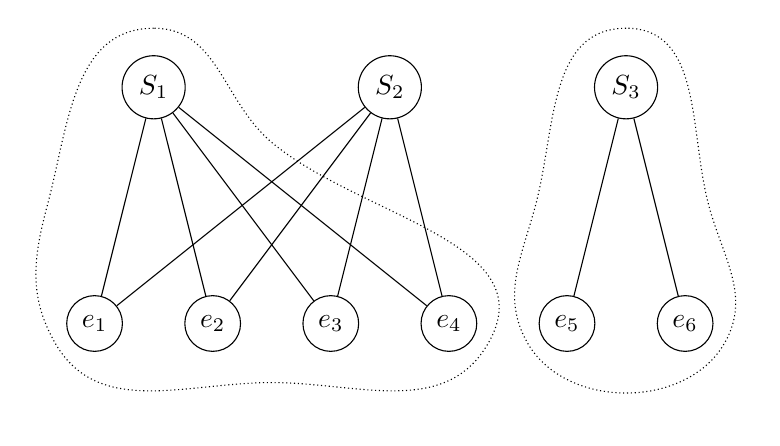
\begin{tikzpicture}
            \draw
                (0.75, 0) node (s1) [draw, circle, minimum size = 2em] {$S_1$}
                (3.75, 0) node (s2) [draw, circle, minimum size = 2em] {$S_2$}
                (6.75, 0) node (s3) [draw, circle, minimum size = 2em] {$S_3$}
                
                (0,   -3) node (e1) [draw, circle, minimum size = 2em] {$e_1$}
                (1.5, -3) node (e2) [draw, circle, minimum size = 2em] {$e_2$}
                (3,   -3) node (e3) [draw, circle, minimum size = 2em] {$e_3$}
                (4.5, -3) node (e4) [draw, circle, minimum size = 2em] {$e_4$}
                (6,   -3) node (e5) [draw, circle, minimum size = 2em] {$e_5$}
                (7.5, -3) node (e6) [draw, circle, minimum size = 2em] {$e_6$}

                (s1) edge (e1)
                (s1) edge (e2)
                (s1) edge (e3)
                (s1) edge (e4)
                (s2) edge (e1)
                (s2) edge (e2)
                (s2) edge (e3)
                (s2) edge (e4)
                (s3) edge (e5)
                (s3) edge (e6)
            ;

            \draw[densely dotted] (0.75, 0.75)
                to[out = 180, in = 75]  (-0.6, -1.5) 
                to[out = 255, in = 120] (-0.5, -3.25)
                to[out = 300, in = 180] (2.25, -3.75)
                to[out = 0  , in = 240] (5, -3.25)
                to[out = 60 , in = 320] (2.25, -0.7)
                to[out = 140 , in = 0]  cycle;
            ;

            \draw[densely dotted] (6.75, 0.75)
                to[out = 180, in = 75]  (5.6, -1.5) 
                to[out = 255, in = 120] (5.5, -3.25)
                to[out = 300, in = 240] (8, -3.25)
                to[out = 60 , in = 285] (7.8, -1.5)
                to[out = 105 , in = 0]  cycle;
            ;

        \end{tikzpicture}
        \caption{Graph representation of a Max Cover instance, $k \leq 2$}
        \label{fig:mcp-ex1}
    \end{figure}
\end{example}

The Max Cover problem is known to be \np-hard, however, an algorithm has been designed that makes a good approximation for the optimal solution:

\noindent\begin{minipage}{\linewidth}
    \begin{lstlisting}[caption = {The Greedy algorithm to solve the densest subgraph problem}, label = {lst:mcp-greedy}]
algorithm $\mcgre(S, k)$:
    $T \gets \emptyset$
    for $i = 1, \ldots, k$:
        let $A \in S$ be a set that maximizes $\abs{\bigcup_{S_i \in T} S_i \cup A}$
        $T \gets T \cup \{A\}$
        $S \gets S \setminus \{A\}$
    return $T$
    \end{lstlisting}
\end{minipage}

The essential idea is that on each iteration, of all the remianing subsets in $S$, the picked subset $A$ is the one that, along with the current state of $T$, increases the coverage more than the others, effectively maximizing the next iteration of $T$. Another way of seeing this operation is that, at each step, the algorithm removes the nodes already covered by $T$, before choosing the next $A$.

Before delving into the related theorems, some specific notion are introduced which will help later. Also, for the sake of referring to specific states of objects during the execution of the algorithm, the state of object $T$ at iteration $i$ will be denoted as $T^{(i)}$. Let $f$ be the function counting the total elements covered by a family of subsets $T$:

\[
    f(T) = \abs{\bigcup T}
\]

\begin{definition}[Incremental gain]\label{def:incremental-gain}
    Given a subset $A$ and a family of subsets $T$, the \emph{incremental gain} of $A$ on $T$ is the number of new elements that are covered with $A$ that weren't covered before adding it to the family $T$:
    \[
        \incr(A, T) = \abs{A \setminus \bigcup T}
    \]
    In terms of the function $f$:
    \begin{equation}\label{eq:mcp-dsa}
        \incr(A, T) = f(\{A\} \cup T) - f(T)
    \end{equation}
\end{definition}

\begin{proposition}[Diminishing returns]\label{prop:mcp-dimret}
    Given two subset families $S$ and $T$, for any subset $A$:
    \[
        S \supseteq T \implies \incr(A, S) \leq \incr(A, T)
    \]
\end{proposition}

\begin{proposition}\label{prop:mcp-greediness}
    The greediness of $\mcgre$ can be formalized as follows:
    \[
        \forall A \in S\; \forall 0 \leq i \leq k - 1 \qquad \incr(A, T^{(i)}) \leq \incr(A^{(i + 1)}, T^{(i)})
    \]
\end{proposition}

\begin{theorem}\label{thm:mcp-greedy}
    The algorithm $\mcgre$, described in [\ref{lst:mcp-greedy}], returns a $\left(1-\frac{1}{e}\right)$-approximation for max cover.
\end{theorem}

\begin{proof}
    Fix an optimal solution $T^* = \{S_1^*, S_2^*, \ldots, S_k^*\}$; for ease of writing, the first $i$ subsets of $T^*$ will be denoted as $T^*[i]$, for any $i$. Recall to not confuse this with $T^{(i)}$, which denotes the state of $T$ during algorithm execution at iteration $i$.

    \begin{lemma}\label{l:mcp-1}
        \[
            \forall\ 0 \leq i \leq k - 1 \quad OPT = f(T^*) \leq f(T^{(i)}) + k \cdot \left( f(T^{(i + 1)}) - f(T^{(i)}) \right)
        \]
    \end{lemma}

    \begin{proof}
        \begin{align*}
                  f(T^*)
            &\leq f(T^* \cup T^{(i)}) & \text{(by optimality of of $T^*$)}&\\
            &=    f(T^* \cup T^{(i)}) + \sum_{j = 0}^{k - 1} \left( f(T^*[j] \cup T^{(i)}) - f(T^*[j] \cup T^{(i)}) \right)         & \text{(zero sum)} \\
            &=    f(T^*[0] \cup T^{(i)}) + \sum_{j = 0}^{k - 1} \left( f(T^*[j + 1] \cup T^{(i)}) - f(T^*[j] \cup T^{(i)}) \right)  & (T^*[k] = T^*) \\
            &=    f(T^{(i)}) + \sum_{j = 0}^{k - 1} \left( f(T^*[j + 1] \cup T^{(i)}) - f(T^*[j] \cup T^{(i)}) \right)              & (T^*[0] = \emptyset) \\
            &=    f(T^{(i)}) + \sum_{j = 0}^{k - 1} \incr \left( S^*_{j + 1}, T^*[j] \cup T^{(i)} \right)                           & \left( \begin{aligned} \text{by $\incr$ definition [\ref{eq:mcp-dsa}]} \\ T^*[j + 1] \setminus T^*[j] = S^*_{j + 1} \end{aligned} \right) \\
            &\leq f(T^{(i)}) + \sum_{j = 0}^{k - 1} \incr \left( S^*_{j + 1}, T^{(i)} \right)                                       & \text{(by proposition [\ref{prop:mcp-dimret}])} \\
            &=    f(T^{(i)}) + \sum_{j = 1}^k \incr \left( S^*_j, T^{(i)} \right)                                                   & \text{(index shift)} \\
            &\leq f(T^{(i)}) + \sum_{j = 1}^k \incr \left( A^{(i + 1)}, T^{(i)} \right)                                             & \text{(by proposition \ref{prop:mcp-greediness})} \\
            &=    f(T^{(i)}) + k \cdot \incr \left( A^{(i + 1)}, T^{(i)} \right)                                                    & \\
            &=    f(T^{(i)}) + k \cdot \left( f(T^{(i + 1)}) - f(T^{(i)}) \right)                                                   & \left( T^{(i + 1)} = T^{(i)} \cup A^{(i + 1)} \right)
        \end{align*}
    \end{proof}

    What lemma [\ref{l:mcp-1}] essentially proves is that, at each iteration, the partial solution $T^{(i)}$ held by the algorithm enforces an upper bound for the partial optimal solutions.
    
    Now it is desirable to prove that such excess, $k \cdot \left( f(T^{(i + 1)}) - f(T^{(i)}) \right)$, shrinks as the algorithm proceeds with its iterations. Define the difference between the optimal solution and the partial solution at time $i$ as $\delta_i := f(T^*) - f(T^{(i)})$.
    
    \begin{observation}\label{obs:mcp-1}
        $\delta_i - \delta_{i+1} = f(T^*) - f(T^{(i)}) - \left( f(T^*) - f(T^{(i + 1)}) \right) = f(T^{(i + 1)}) - f(T^{(i)})$.
    \end{observation}
    
    \begin{lemma}\label{l:mcp-2}
        The difference between the optimal solution and the partial solution at time $i$ decreases as $i$ increases:
        \[
            \delta_{i + 1} \leq \left( 1 - \frac{1}{k} \right) \delta_i
        \]
    \end{lemma}
    \begin{proof}
        \begin{align*}
            f(T^*) - f(T^{(i)})     \leq&\ k \cdot \left( f(T^{(i + 1)}) - f(T^{(i)}) \right)   & \text{(by lemma [\ref{l:mcp-1}])} \\
            \delta_i                \leq&\ k \cdot \left( f(T^{(i + 1)}) - f(T^{(i)}) \right)   & \\
            \delta_i                \leq&\ k \cdot \left( \delta_i - \delta_{i + 1} \right)     & \text{(by observation [\ref{obs:mcp-1}])} \\
            k \cdot \delta_{i + 1}  \leq&\ k \cdot \delta_i - \delta_i                          & \\
            k \cdot \delta_{i + 1}  \leq&\ (k - 1) \cdot \delta_i                               & \\
            \delta_{i + 1}          \leq&\ \left( 1 - \frac{1}{k} \right) \delta_i              & 
        \end{align*}
    \end{proof}

    \begin{corollary}
        \[
            \delta_k \leq \left( 1 - \frac{1}{k} \right)^k \delta_0 = \left( 1 - \frac{1}{k} \right)^k f(T^*)
        \]
    \end{corollary}

    Therefore:
    \begin{align*}
        f(T^*) - f(T^{(k)}) \leq&\ \left( 1 - \frac{1}{k} \right)^k f(T^*)              & \\
        \left( 1 - \left( 1 - \frac{1}{k} \right)^k \right) f(T^*) \leq&\ f(T^{(k)})    & \\
        \left( 1 - \frac{1}{e} \right) f(T^*) \leq&\ f(T^{(k)})                         & \text{(by limit [\ref{eq:limit-1/e}])} \\
    \end{align*}
    Since $f(T^{(k)})$ is the subset returned by the algorithm $\mcgre$, the proof is complete.
\end{proof}

\begin{corollary}
    $\mcgre$ is optimal: it gives the best possible approximation to the max cover problem.\footnote{The best approximation efficiently obtainable for any submodular-related problem is proven to be up to a factor of $\left( 1 - \frac{1}{e} \right)$}
\end{corollary}

Note that this algorithm returns a pretty good approximation of the optimal solution even after only half of the $k$ iterations: the approximation factor incurred by performing all $k$ steps is $1 - \frac{1}{e} \simeq 0.632$, whereas performing only half of the total steps shrinks it to $1 - \frac{1}{e}^{\frac{1}{2}} \simeq 0.393$. This result is extraordinarily useful especially when a maximum iteration count $k$ is not given. Perhaps surprisingly, $\mcgre$ gives a useful approximation even at the first iteration:
\[
    f(T^*) - f(T^{(1)}) = \delta_1 \leq \left( 1 - \frac{1}{k} \right) f(T^*) \quad \implies \quad f(T^{(1)}) \geq \frac{1}{k} f(T^*)
\]

This is because the first set picked by the algorithm is essentially the one with largest cardinality; also, if $k = 1$ then such solution would trivially be optimal.

\section{Submodular functions}

Let $f: \powerset(U) \to \real$ be a function on sets:

\begin{definition}[Modular function]\label{def:modular}
    $f$ is modular if, $\forall\ S, T \subseteq [n]$,
    \begin{equation}\label{eq:modular}
        f(S) + f(T) = f(S \cup T) + f(S \cap T).
    \end{equation}
\end{definition}

\begin{definition}[Submodular function]\label{def:submodular}
    $f$ is submodular if, $\forall\ S, T \subseteq [n]$,
    \begin{equation}\label{eq:submodular}
        f(S) + f(T) \geq f(S \cup T) + f(S \cap T).
    \end{equation}
\end{definition}

\begin{definition}[Supermodular function]\label{def:supermodular}
    $f$ is supermodular if, $\forall\ S, T \subseteq [n]$,
    \begin{equation}\label{eq:supermodular}
        f(S) + f(T) \leq f(S \cup T) + f(S \cap T).
    \end{equation}
\end{definition}

\begin{example}[Modular function]
    Set cardinality as a function is modular:
    \begin{itemize}
        \item $f(S) = |S|$ and $f(T) = |T|$,
        \item $f(S \cap T) = |S \cap T|$,
        \item $f(S \cup T) = |S \cap T| + |S \symdiff T|$,
        \item $f(S) + f(T) = 2 |S \cap T| + |S \symdiff T|$,
        \item $2 |S \cap T| + |S \symdiff T| = |S \cap T| + |S \cap T| + |S \symdiff T|$.
    \end{itemize}    
\end{example}

\begin{example}[Submodular function]
    The coverage function [\ref{eq:coverage}] is submodular:
    \begin{itemize}
        \item let $S=\{\{1,2\}\}$ and $T = \{\{1\}\}$
        \item $f(S)=2$ and $f(T)=1$,
        \item $f(S \cap T) = 0$,
        \item $f(S \cup T) = 2$,
        \item $f(S) + f(T) = 3$,
        \item $3 > 2$.
    \end{itemize}    
\end{example}

\begin{theorem}\label{thm:modular}
    $f(S)$ is modular iff $\exists\ z, w_1, \ldots, w_{|S|}$ such that
    \begin{equation}
        f(S) = z + \sum_{i \in S} w_i.
    \end{equation}
\end{theorem}

\todo{Unproven}


\subsection{Submodular functions properties} \label{sec:submodular-properties}

Here, the definition of incremental gain given back in \ref{def:incremental-gain} is carried over

\begin{lemma}[Submodular diminishing returns] \label{lem:dim-return}
    Proposition [\ref{prop:mcp-dimret}] is actually applicable to any submodular function $f$, with the added constraint that the objects $A$ must not be in $T$:
    \[
        S \subseteq T \quad \implies \quad \forall A \not\in T \; \incr (A, S) \geq \incr(A, T)
    \]
\end{lemma}

\begin{proof}
    Starting from the submodular inequality, the two families that give the result of interest are $T$ and $S \cup \{A\}$:
    \begin{align*}
        f(S \cup \{A\}) + f(T)  &\geq f((S \cup \{A\}) \cup T) + f((S \cup \{A\}) \cap T)   & \text{(by definiton of submodular function)} \\
        f(S \cup \{A\}) + f(T)  &\geq f(T \cup \{A\}) + f(S)                                & \\
        f(S \cup \{A\}) - f(S)  &\geq f(T \cup \{A\}) - f(T)                                & \\
        \incr (A, S)            &\geq \incr(A, T)                                           & \text{(by definition of incremental gain)} \\
    \end{align*}
\end{proof}

The lemma is actually proven to work both ways; the reverse implication is left to prove as an exercise. Also, if $f$ is modular, the equality holds instead.

\begin{lemma}\label{lem:submodular-power-function}
    Let $f_i$ be a collection of $k$ submodular functions, and $\alpha_i$ a corresponding collection of nonegative reals. Then their linear combination $g$ is also submodular:
    \[
        g(S) = \sum_{i = 1}^k \alpha_i f_i(S)
    \]
\end{lemma}

\begin{proof}
    \begin{align*}
               g(S) + g(T) 
           =&\ \sum_{i = 1}^k \left( \alpha_i f_i(S) \right) + \sum_{i = 1}^k \left( \alpha_i f_i(T) \right)                & \\
           =&\ \sum_{i = 1}^k \alpha_i \left( f_i(S) + f_i(T) \right)                                                       & \\
        \geq&\ \sum_{i = 1}^k \alpha_i \left( f_i (S \cap T) + f_i (S \cup T) \right)                                       & \text{(by submodularity)} \\
           =&\ \sum_{i = 1}^k \left( \alpha_i f_i(S \cap T)\right) + \sum_{i = 1}^k \left( \alpha_i f_i (S \cup T) \right)  & \\
           =&\ g(S \cap T) + g(S \cup T)                                                                                    &
    \end{align*}
    
    Note that if negative coefficients $\alpha_i$ are introduced, the lemma fails.
\end{proof}


\subsection{One particular submodular function}

\begin{definition}\label{def:fca}
    Let $w$ be a function that assigns a nonnegative weight on all subsets of a subset family $T$. Define the function:
    \[
        f_w(A) = \sum_{\substack{S \in T \\ S \cap A \neq \emptyset}} w(S)
    \]
\end{definition}

This function sums the weights of the subsets intersecting the given set $A$.

\begin{example}
    Let $T = \{\{1, 2\}, \{2, 3\}\}$, $w(\{1, 2\}) = 1$, $w(\{2, 3\}) = 3$. Then $f_w(\{1\}) = 1$ and $f_w(\{2\}) = 4$.
\end{example}

Note how this function is similar to the coverage function [\ref{eq:coverage}].

\begin{lemma} \label{lem:fC-submodular}
    $f_w$ is submodular.
\end{lemma}

\begin{proof} 
    Given $A$ and $B$ two subset families, partition $T$ in blocks based on whether the subsets contained in $T$ are disjoint from $A$ and/or $B$; in particular: 
    \begin{align*}
        T_A     &= \{S \in T : S \cap A \neq \emptyset \wedge S \cap B = \emptyset\} & \\
        T_B     &= \{S \in T : S \cap A = \emptyset \wedge S \cap B \neq \emptyset\} & \\
        T_{AB}  &= \{S \in T : S \cap A \neq \emptyset \wedge S \cap B \neq \emptyset\} &
    \end{align*}
    
    Since the conditions governing the partition are mutually exclusive, the function images can be reinterpreted in terms of such blocks:
    \begin{align*}
        f_w(A)             =&\ \sum_{S \in T_A} w(S) + \sum_{S \in T_{AB}} w(S)                         & \\
        f_w(B)             =&\ \sum_{S \in T_B} w(S) + \sum_{S \in T_{AB}} w(S)                         & \\
        f_w(A \cup B)      =&\ \sum_{S \in T_A} w(S) + \sum_{S \in T_B} w(S) + \sum_{S \in T_{AB}} w(S) & \\
        f_w(A \cap B)   \leq&\ \sum_{S \in T_{AB}} w(S)                                                 &
    \end{align*}
    Note that the last image is not an equality because, in general, while a set $C$ in $T_{AB}$ does intersect both $A$ and $B$, it may also be simultaneously disjoint from $A \cap B$ as shown in figure \ref{fig:sets-intersect-empty}, and thus would not add its weight in $f_w(A \cap B)$.

    \begin{figure}[ht]
        \centering
        \begin{tikzpicture}
            \path[radius = 2.2]
                (0, -2.2) node (c) {$C$}
                arc[start angle = 270, end angle = 150] node (a) {$A$}
                arc[start angle = 150, end angle = 30] node (b) {$B$}
            ;
            \draw
                (a) circle (2)
                (b) circle (2)
                (c) circle (2)
            ;
        \end{tikzpicture}
        \caption{An instance where $C$ intersects $A$ and $B$ and is disjoint from $A \cap B$}
        \label{fig:sets-intersect-empty}
    \end{figure}
    
    Adding $f_w(A)$ and $f_w(B)$ together in terms of the above sums:
    \begin{align*}
               f_w(A) + f_w(B) 
           =&\ \sum_{S \in T_A} w(S) + \sum_{S \in T_B} w(S) + 2 \sum_{S \in T_{AB}} w(S)   & \\
           =&\ f_w(A \cup B) + \sum_{S \in T_{AB}} w(S)                                     & \\
        \geq&\ f_w(A \cup B) + f_w(A \cap B)                                                & 
    \end{align*}
    which is indeed the submodular inequality for $f_w$.
\end{proof}

Note that for very large subsets families $T$, computing $f_w$ becomes impractical, because it requires computing a sum on each single subset in $T$.


\section{\textsc{Kkt} model}

%This model has been designed by Kempe, Kleinsberg and Tardos, and has the purpose of .

This case study is about product giveaway for advertising purposes: assume there is a stock of $k$ products, and $k$ persons receive one each; the goal of such is to spread information about the product starting from the former $k$ persons. The model is constructed from the following rules:

\begin{itemize}
    \item the social network is modeled by an undirected graph;
    \item \emph{influential} nodes are those with high degree;
    \item each person receiving a product keeps it forever;
    \item the information spread takes place in discrete time steps:
    \begin{itemize}
        \item at time $t_0$, the only persons having knowledge the product are those that received it during the giveaway;
        \item at time $t_i$, for each of the edges incident on the nodes knowing the product, a coin is flipped: with prob $p$ the information will spread on such edge, otherwise the edge is removed from the graph.
    \end{itemize}  
\end{itemize} 

Despite the model having an apparent temporal nature, note that each edge in the network gets to flip exactly one coin regardless of when it is actually flipped, and all coin throws are independent. This makes it equivalent to flip all coins at once, and by looking at the components of the resulting graph:
\begin{itemize}
    \item each component containing at least one starting node will be completely informed;
    \item the others will be oblivious.
\end{itemize}

Knowing the final components makes picking the right starting nodes simple: sort the components by decreasing size and pick one node for each of the first $k$ components. However, this is not the case because the starting nodes must be chosen beforehand.

Nevertheless, this conundrum can be solved in a probabilistic way. Consider an instance of this problem, throw all the coins, and let $A \subseteq E(G)$ be the set of edges that are not removed from the graph, and $T_A$ the partition of the nodes grouping them into the resulting connected components. Let $R(S)$ be the set of nodes informed by the starting nodes in $S$; this is clearly a random variable depending on which edges survive. Now it is possible to comput the expected cardinality of the reached set $R(S)$ conditioned on the edge set $A$, which is what the original problem wants to maximize:

\[
    \expect(\abs{R(S)} \knowing A) = \sum_{\substack{S_i \in T_A \\ S_i \cap S \neq \emptyset}} \abs{S_i}
\]

\begin{claim}
    Let $f_A(S)$ be the expected reach $\expect(\abs{R(S)} \knowing A)$ of a \textsc{kkt} instance parameterized by $S$. Then $f_A$ is submodular. 
\end{claim}

\begin{proof}
    Note how the definition of $f_A$ is much similar to the function $f_w$ defined in \ref{lem:fC-submodular}; the only difference is in the weight function $w$ of $f_w$ being the set cardinality in $f_A$
\end{proof}

Moreover, the conditioning by $A$ in $f_A$ can be removed by total expectation:
\begin{equation}\label{eq:sub-fs}
    \expect(\abs{R(S)}) = \sum_{A \subseteq E} \left( \expect(\abs{R(S)} \knowing A) \cdot \Pr[A] \right) = \sum_{A \subseteq E} \left( f_A(S) \cdot \Pr[A] \right) = f(S)
\end{equation}

\begin{claim}
    $f$ is submodular.
\end{claim}
\begin{proof}
    $f$ is by definition a nonnegative linear combination of submodular functions; by lemma \ref{lem:submodular-power-function}, $f$ is submodular too.
\end{proof}

\todo{Elaborate better

The problem in optimizing this function is that computing it on a single set takes exponential time, but it can be approximated very well; as an exercise you can try to give the best sampling algorithm to do it (hint: an approximation can be obtained by using [\ref{eq:chebyshev}]). Note that it is possible to compute the average among the various results because the value of $f(S)$ is bounded between $k$ and $n$.
}

\section{A greedy algorithm for submodular functions.} \label{sec:submodular-greedy}

The algorithm used to solve the Max cover problem can be refined and generalized to work for any monotone, nonnegative submodular function function $f$, with some tweaks:

\begin{lstlisting}[caption = {Greedy algorithm for submodular functions}, label = {lst:fS-greedysm}]
algorithm $\subgre(f, \varepsilon, S, k)$:
    $T \gets \emptyset$
    for $i = 1, \ldots, k$:
        let $A \in S$ be such that $\incr_f(A, T) \geq (1 - \varepsilon) \cdot \max_{S_i \in S} \left( \incr_f(S_i, T) \right)$
        $T \gets T \cup \{A\}$
        $S \gets S \setminus \{A\}$
    return $T$
\end{lstlisting}

Apart from the new parameters that convey the generalization of the algorithm, the relevant tweak consists in picking the subset $A$ that is a $(1 - \varepsilon)$-approximation ot the optimal, instead of just maximizing $f(A)$.

\begin{proposition}\label{prop:subgreediness}
    The greediness of $\subgre$ can be formalized as follows:
    \[
        \forall A \in S\; \forall 0 \leq i \leq k - 1 \qquad \incr \left( A, T^{(i)} \right) \leq \oneover{1 - \varepsilon} \cdot \incr \left( A^{(i + 1)}, T^{(i)} \right)
    \]
\end{proposition}

\begin{theorem}\label{thm:sub-greedy}
    If $f$ is monotone, non-negative and submodular, then Greedy returns a $(1 - e^{\varepsilon - 1})$-approximation. Note that $1 - e^{\varepsilon - 1} = 1 - \oneover{e} - O(\varepsilon)$.
\end{theorem}

\begin{proof}
    Let $T^* = \{S_1^*, S_2^*, \ldots, S_k^*\}$ be an optimal solution. By reusing some findings in the proof of lemma \ref{l:mcp-1}, for any iteration $i$:
    \begin{align*}
                   f(T^*) 
            \leq&\ f(T^{(i)}) + \sum_{j = 1}^k \incr \left( S^*_j, T^{(i)} \right)                                          & \text{(by proof of lemma [\ref{l:mcp-1}])} \\
            \leq&\ f(T^{(i)}) + \sum_{j = 1}^k \oneover{1 - \varepsilon} \cdot \incr \left( A^{(i + 1)}, T^{(i)} \right)    & \text{(by proposition [\ref{prop:subgreediness}])} \\
               =&\ f(T^{(i)}) + \frac{k}{1 - \varepsilon} \cdot \incr \left( A^{(i + 1)}, T^{(i)} \right)                   &
    \end{align*}

    \todo{Unfinished, may need to translate some more of the proof of theorem \ref{thm:mcp-greedy}}
\end{proof}